\newpage
\subsection{Resultados}

\label{subsection:resultados}
	tablas, gráficos, análisis y recomendaciones
	\begin{itemize}
		\item Aca debería explicar como fueron procesados los
                  resultados y que tipo de resultados se van a mostrar (ej. los
                  que tuvieron mejor y peor performance). \JS{hay que empezar a
                  poner cuales se van a mostrar y discutir}
                \item \JS{Baseline. Comparar con Wang}
		\item Resultados de dataset con imagenes reales.
		\begin{itemize}
			\item Se presentan los mejores resultados y los parámetros con los cuales se obtuvieron. Se van a presentar los gráficos de los 2 mejores resultados junto con sus matrices de confusión.
			\item Idem pero con los peores resultados obtenidos.
		\end{itemize}
		\item Idem con dataset sintéticos
		\item Idem con dataset sintéticos + reales.

	\end{itemize}
	
		
	Esta subsección está dividida en cuatro partes. La primera etapa, está dedicada a mostrar los resultados obtenidos de haber realizado experimentos basándonos en los parámetros obtenidos del trabajo de Wang et al. sobre nuestra implementación del mismo. Estos valores van a conformar los baselines para los siguientes experimentos. 
	
	La segunda, corresponde a los resultados obtenidos de haber entrenado y evaluado el clasificador Random Ferns con imágenes de caracteres en escenas naturales. Los gráficos mostrados en esta parte reflejan la relación entre la dimensión de los grupos y la precisión del clasificador.
	
	La tercera etapa contiene los resultados de haber reemplazado las imágenes reales del conjunto de entrenamiento por un conjunto de imágenes sintéticas (ver \ref{subsubsection:recon-caracteres}). El objetivo es demostrar como influye en la performance de clasificación al entrenar al clasificador con imágenes sintéticas.
	
	En la última parte, se procederán a mostrar los resultados de haber modificado al conjunto de entrenamiento de la segunda parte agregándole en diferentes proporciones imágenes sintéticas. Se compara este último enfoque con los anteriores para ver el impacto que produce en la performance dicho cambio.
	
	\subsubsection{Resultados de la implementación propia}
	
	Basados en el paper de Wang et al., se propuso realizar una reimplementación del trabajo realizado por los autores. Teniendo en cuenta los siguientes parámetros conocidos: cantidad de grupos = $256$ y bits por grupo = $6$ (con lo cual obtenemos vectores de características de longitud $1536$), se obtuvieron los resultados que se pueden apreciar en la tabla \ref{table: Baseline-Table}. En la misma, expresamos con ``NATIVE+FERNS'' los resultados obtenidos al haber entrenando y evaluando al clasificador Random Ferns con imágenes reales. De la misma manera, ``SYNTH+FERNS'' refiere a los experimentos donde se usaron $1000$ imágenes sintéticas durante el entrenamiento.
	
	\begin{table}
		\centering
	    \begin{tabular}{ | l | l | l | p{5cm} |}
    			\hline
    				\textbf{Implementación} & \textbf{Score} \\ \hline
    				Wang NATIVE+FERNS & 0.54\% \\ \hline
    				Impl. propia NATIVE+FERNS & 0.50\% \\ \hline
    				Wang SYNTH+FERNS & 0.47\% \\ \hline
    				Impl. propia SYNTH+FERNS & 0.43\% \\
    				
    			\hline
    		\end{tabular}	
    		\caption[Resultados reales y sintéticas para baseline]{Resultados obtenidos en la reimplementación del trabajo de Wang et al.}
    		\label{table: Baseline-Table}
	\end{table}
	
	Como se puede ver en base a los resultados expuestos en la tabla \ref{table: Baseline-Table}, hay diferencias significativas entre los resultados de ambas implementaciones que se deben a varios factores. Existen ciertos parámetros que no están especificados en el trabajo de Wang et al. como es el caso del método de binarización utilizado. Habiendo leido la implementación de los autores, se propuso como método de binarización, la generación de variables aleatorias uniformes. Este enfoque resultó ser el más adecuado debido a que es el que más se asemeja a lo que hicieron los autores en \cite{wang}.	Otro parámetro no especificado fue el valor de \textit{alpha} para la inicialización de las tablas el cual influye en la performance si no se elige bien. Asi mismo, la implementación de HOG que usan los autores es la desarrollada por Piotr Dollár la cual es una variación del método original propuesto por Dalal \& Triggs en \cite{DT05}. En la reimplementación se utiliza la función HOG extraida de una librería de python llamada scikit-images, la cual está basada en \cite{DT05} pero difiere de la usada por los autores. Una de las diferencias entre ambas funciones está en que la desarrollada por Piotr Dollar acepta imágenes a color y la que se usa en este trabajo sólo acepta imágenes en escala de grises.
	
	Ante esta situación se decide por establecer como baselines los resultado obtenidos por la configuración más cercana a la usada en \cite{wang}. Teniendo en cuenta los parámetros conocidos, se establecen además los siguientes: $8$ orientaciones y $9$ celdas por bloque para la función HOG; la generación de variables aleatorias uniformes entre dos puntos \textit{a} y \textit{b} como método para la binarización. Por último, el valor de alpha se estableció en $0.01$ pués es el valor que más impacto produjo en estos experimentos.
	
	En la siguiente sección, donde se experimentan con imágenes reales, se va a tomar como baseline el valor $0.50$. De la misma manera, en los experimentos con imágenes sintéticas, el baseline pasará a ser $0.43$. Por último, en la sección sobre los experimentos con conjuntos de entrenamiento mixtos se van a mostrar ambos baselines.

	\subsubsection{Imágenes Reales}
	
	En esta parte se van a mostrar cinco gráficos. Los primeros 4 corresponden a los métodos utilizados en la binarización con lo cual se busca ver cual de los 4 arroja mejores resultados. Además, los primeros cuatro resultados reflejan la diferencia en performance al considerar grupos de diferente dimensión $\in \{ 1, 2, 4, 8, 10, 12\}$. Con esto buscamos establecer para cada caso, qué dimensión arroja los mejores resultados. Cabe aclarar que cada gráfico refleja la media de los resultados de 5 corridas del experimentos junto con la desviación estandard asociada. El quinto gráfico \ref{fig: Reales-Comparativa metodos} reune los mejores resultados de clasificación de los cuatro primeros, para establecer una comparación más precisa. La tabla \ref{table: reales-comparativa} se muestra un resumen de los mejores valores.
	
	 Dada la gran cantidad de parámetros que se manejan en estos experimentos, se va a intentar dejar detallado en el análisis cuales son los mejores y se los va a usar para los siguientes experimentos.
		
			\begin{figure}[htbp!]
				\centering
				\subfloat[Resultados usando la media \label{fig: Reales-media}]{
					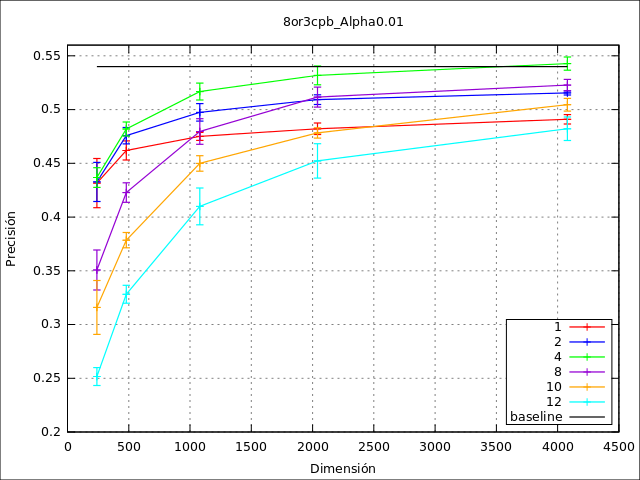
\includegraphics[width=8cm]{img/resultados/reales/mean.png}
				}
				\subfloat[Resultados usando la mediana \label{fig: Reales-mediana}]{
					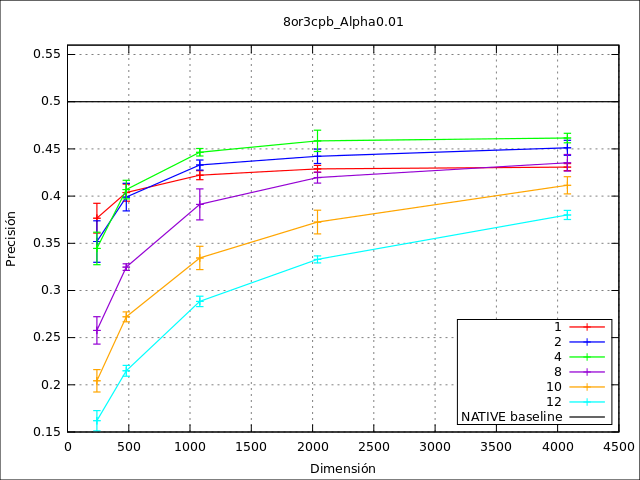
\includegraphics[width=8cm]{img/resultados/reales/median.png}
				}
				\\
				\subfloat[Resultados usando la distribución exponencial \label{fig: Reales-expon}]{
					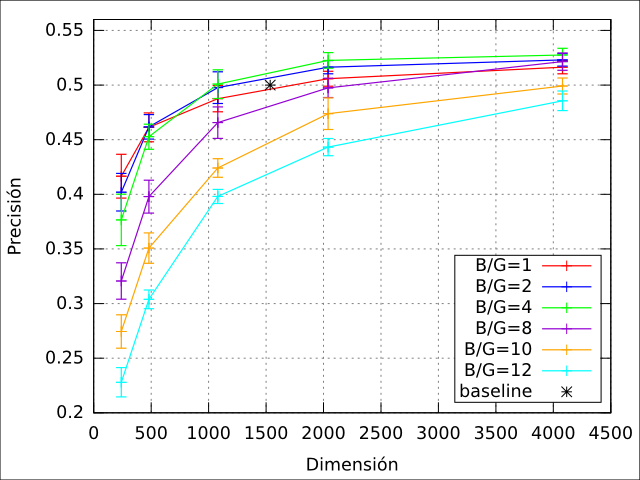
\includegraphics[width=8cm]{img/resultados/reales/expon.png}
				}
				\subfloat[Resultados usando bootstrap\label{fig: Reales-bootstrap}]{
					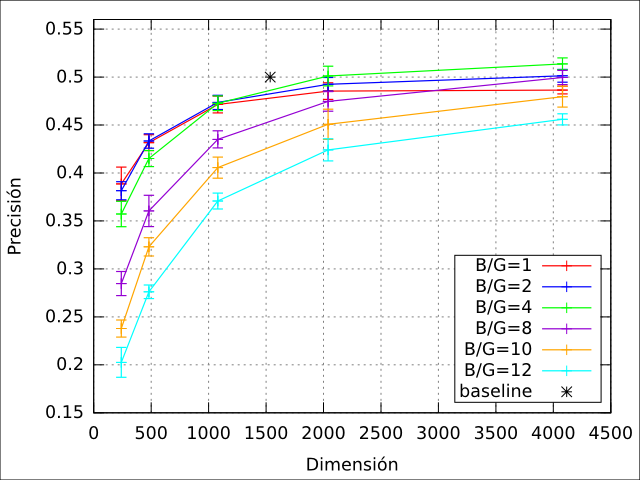
\includegraphics[width=8cm]{img/resultados/reales/bootstrap.png}
				}
				\caption[Resultados-Reales]{Esta figura presenta los resultados obtenidos por los 4 métodos propuestos para la binarización de los vectores.}
				\label{fig: Resultados-Reales}
			\end{figure}
			
	Teniendo en cuenta los resultados en \ref{fig: Resultados-Reales}, a simple vista se puede observar que los resultados obtenidos usando la media como método para binarizar los vectores son los mejores, llegando estos a un máximo cercano al $55\%$ de precisión. En el caso opuesto, el usar la mediana arrojó los peores resultados ya que en el mejor de los casos se supera el $47\%$ a diferencia de bootstrap que llega a $51\%$ . El uso de la distribución exponencial en los casos donde la longitud de los grupos es baja ($1$, $2$ bits por grupo) supera a la media en performance pero se mantiene por debajo a medida que aumentamos este valor (casos $\{ 4, 8, 10, 12\}$ bits por grupo). Los valores que podemos encontrar en \ref{fig: Reales-expon} se acercan a los del a media llegando a un máximo en la precisión de $53\%$. En cuanto al uso de bootstrap, se puede apreciar que los resultados se mantienen por debajo de los obtenidos con la distribución exponencial y la media con puntajes que rondan entre $45\%$ y $52\%$.
	
	En cuanto a las dimensiones evaluadas $\{ 240, 480, 1080, 2040, 4080 \}$ es claro que a medida que aumentamos la longitud de los vectores aumenta la performance. Se puede ver que, cuando se usan vectores de longitud reducida (en este caso $240$), se marca una diferencia importante en la precisión entre los experimentos realizados con grupos de dimensionalidad baja $\{ 1, 2, 4 \}$ y alta $\{8, 10, 12\}$. Es decir, dejando fija la dimensión de los vectores en $240$, mientras más chico es el tamaño de los grupos mejor es el resultado (se puede observar en cualquiera de los gráficos en \ref{fig: Resultados-Reales}). En el otro extremo, si usamos grupos de $12$ bits la precisión baja bastante. La misma relación se mantiene a medida que aumentamos el tamaño de los vectores de características hasta cierto punto. Por ejemplo, en \ref{fig: Resultados-Reales} y específicamente en \ref{fig: Reales-media} es claro que a partir del uso de $1080$ como tamaño de vector en adelante, el uso de grupos de longitud mayor arroja mejores resultados. Lo mismo sucede en las otras figuras en diferentes puntos. En cuanto al uso del valor $4080$, se puede ver que no hay un aumento considerable en la performance que lo diferencie del uso de $2040$. Con esto en mente, es conveniente hacer uso de este último valor ya que otorga resultados similares a los calculados con $4080$ usando vectores mucho más chicos incrementando la eficiencia en el cómputo.
	
	El problema con los vectores binarizados de dimensión reducida, es que almacenan menos información sobre la imagen a comparación de los vectores cuya longitud es mayor. Tal es el caso como se puede observar en \ref{fig: Resultados-Reales}. 
	
	Otro parámetro a analizar aquí es \textit{alpha} $\in \{ 0.0001, 0.001, 0.01, 0.1, 1\}$. Los mejores resultados de cada método se dieron cuando el valor de \textit{alpha} se estableció en $0.01$ y son los que se muestran en la figura \ref{fig: Resultados-Reales}. Valores por encima $0.01$ o muy cercanos a 0 no llegaron en los experimentos a igualar la precisión obtenida con el valor de \textit{alpha} elegido. Por cuestiones de espacio se decidió mostrar en esta sección los resultados que se obtuvieron con el mejor valor de \textit{alpha}. El resto de los gráficos se pueden encontrar en el apéndice ``B'' con el resto de los resultados de los experimentos. A medida que incrementamos el valor de \textit{alpha}, 
	
	Al igual que con el parámetro \textit{alpha}, hay $2$ parámetros que se dejaron fijos y son los relacionados con la función de HOG: la cantidad de \textit{orientaciones} y la cantidad de \textit{celdas por bloque}. Se decidió por usar $8$ y $9$ respectivamente ya que dichos valores devuelven los mejores resultados. 
	
			\begin{figure}[htbp]
				\centering
				\centerline{
					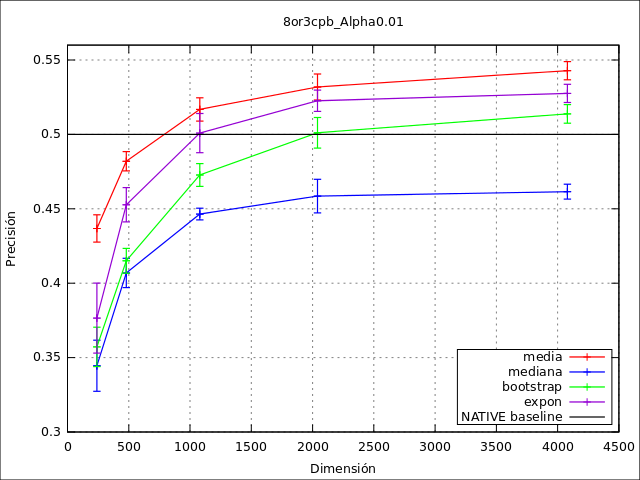
\includegraphics[scale=0.7]{img/resultados/reales/comparativa_metodos.png}
				}
				\caption[Reales comparativa]{El gráfico muestra las mejores curvas de los gráficos presentados en la figura \ref{fig: Resultados-Reales} con la mejor configuración}
				\label{fig: Reales-Comparativa metodos}
			\end{figure}
	
	Del análisis realizado surge que la mejor configuración está dada por \textit{alpha = $0.01$}, \textit{orientaciones = $8$}, \textit{celdas por bloque = $9$}, \textit{bits por grupo = $4$} y \textit{dimensión del vector = 4080}. Se puede observar en \ref{fig: Reales-Comparativa metodos} las mejores curvas para cada método utilizando la mejor configuración (a excepción de la longitud del vector con el objetivo de ver la curva de crecimiento). Queda claro que la media se puede establecer como el mejor método para la binarización por lo cual en los próximos experimentos se procederá a trabajar con el mismo. De la misma manera la mediana termina siendo el peor método. De este último caso se puede ver que incluso para la mejor configuración tiene a ``aplanarse'' a medida que aumentamos la dimensión del vector característica
		
	\begin{table}
		\centering
		\begin{tabular}{ | l | l | l | p{5cm} |}
    			\hline
    				\textbf{NATIVE + FERNS} & \textbf{Score} \\ \hline
    				Media & 0.54\% \\ \hline
    				Mediana & 0.47\%\\ \hline
    				Exponencial & 0.53\% \\ \hline
    				Bootstrap & 0.52\%\\ 
    			\hline
    		\end{tabular}
    		\caption[Resultados imagenes naturales]{Tabla comparativa entre los diferentes métodos propuestos para la binarización en la clasificación de caracteres en escenas naturales.}
    		\label{table: reales-comparativa}
    	\end{table}
    	
    	
    	\newpage
    	\subsubsection{Imágenes Sintéticas}
    	
    En esta etapa se procederán mostrar los resultados obtenidos de los experimentos con las imágenes sintéticas. Además, los gráficos van a representar la relación entre la cantidad de imágenes sintéticas por clase (dado por \textit{IPC} en las siguientes figuras) y la precisión de clasificación dada por los $6$ valores a evaluar que son las dimensiones de los grupos. Teniendo en cuenta los resultados anteriores con las imágenes reales, se decidió por trabajar $8$ orientaciones, $9$ celdas por bloque, alpha de $0.01$ y usando la media como método de binarización ya que son los parámetros que dieron los mejores resultados.
  
			\begin{figure}[htbp]
				\centering
				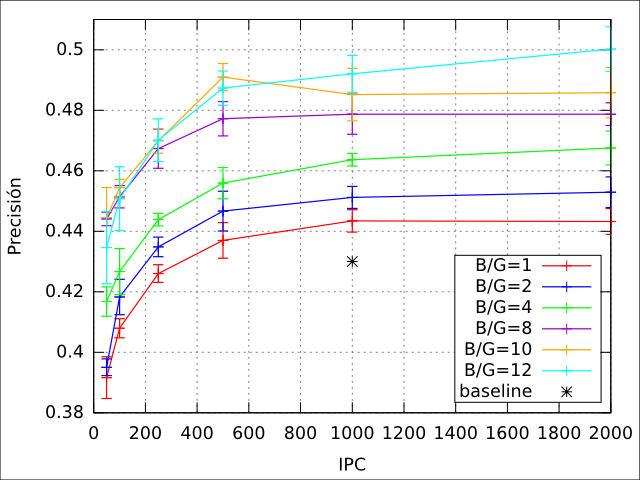
\includegraphics[scale=0.6]{img/resultados/sinteticas/mean_4080.png}
				\caption[Sintéticas media 4080]{El gráfico muestra los resultados obtenidos de haber utilizado la mejor configuración analizada y haciendo uso de vectores binarizados de longitud $4080$}
				\label{fig: Sinteticas-media-4080}
			\end{figure}

			\begin{figure}[htbp]
				\centering
				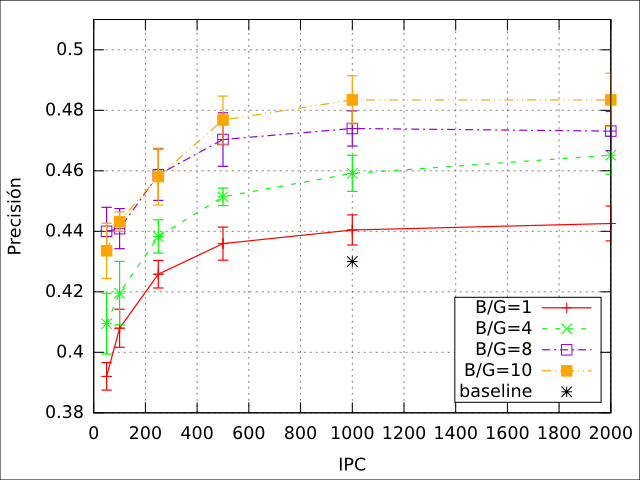
\includegraphics[scale=0.6]{img/resultados/sinteticas/mean_2040.png}
				\caption[Sintéticas media 2040]{EEl gráfico muestra los resultados obtenidos de haber utilizado la mejor configuración analizada y haciendo uso de vectores binarizados de longitud $2040$}
				\label{fig: Sinteticas-media-2040}
			\end{figure}
			
	Hacer texto con las siguientes ideas
	\begin{itemize}
		\item En los experimentos con imágenes sintéticas en general a más cantidad de imágenes por clase mayor es la performance de clasificación. Sin embargo llega un punto en que se deja de aumentar la perfomances y en varios casos disminuye despues de cierto punto.
		\item Es claro que para este tipo de experimentos es mejor tener grupos de dimensiones mayores a los propuestos para las imágenes reales. Analizar que los casos donde los grupos tienen 12 bits la performance decae a comparación de los casos donde los mismo tienen 10 bits.
		\item Defenitivamente la mediana y bootstrap no son buenos métodos para binarizar.
	\end{itemize}
			
\newpage
    	\subsubsection{Imágenes Reales y Sintéticas}
    	
	Por último se van a mostrar los resultados correspondientes de haber entrenado al clasificador con conjuntos de entrenamiento mixtos. Se procederá a mostrar los gráficos con las mejores y peores configuraciones y sus resultados. También se mostrarán las matrices de correlación para todos estos casos. Teniendo en cuenta el análsis anterior, se van a mostrar los resultados de haber utilizado solamente la la media como umbral ya que fue la que retornó los mejores valores.
	
	El gráfico a continuación presenta el eje \textit{x} en escala logarítmica para poder apreciar mejor las variaciones que se dan al experimentar con valores cercanos entre sí.
	
			\begin{figure}[!htbp]
				\centering
				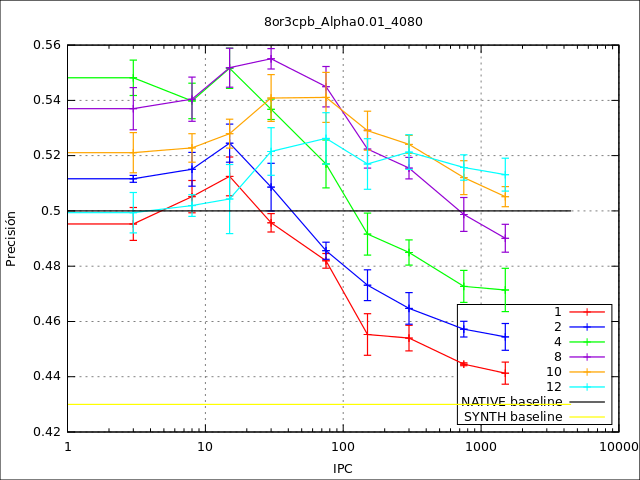
\includegraphics[scale=0.6]{img/resultados/mixtas/best_mean.png}
				\caption[Mixtas media mejor resultado]{El gráfico muestra la configuración que devolvió los mejores resultados.}
				\label{fig: Mixtas-media-mejor}
			\end{figure}

	De la figura \ref{fig: Mixtas-media-mejor} se puede desprender el siguiente análisis. El primero, y uno de los más importantes, hace referencia a la influencia en la clasificación de ir agregando de manera incremental imágenes sintéticas durante la etapa de entrenamiento. Se puede observar que a nivel general todos los experimentos llegaron a un punto donde su performance se desplomó al seguir agregando imágenes sintéticas en el entrenamiento. Sin embargo, este cambio ocurrio en diferentes momentos dependiendo del caso. Por ejemplo, cuando trabajamos con grupos de dimensionalidad baja ($1$, $2$ y $4$ bits por grupo), la precisión del clasificador va en aumento hasta que se llega a un máximo correspondiente al haber entrenado al sistema con igual cantidad de imagenes reales y sintéticas. A partir de ese punto el seguir incrementando la proporción de sintéticas sobre reales trajo efectos negativos en los resultados como se puede apreciar en el gráfico presentado. En los casos donde consideramos $10$ y $12$ bits por grupo el rendimiento se desploma cuando consideramos más de 75 imágenes sintéticas. La mejor curva en el gráfico la obtenemos cuando consideramos $8$ bits por grupo y entrenamos al clasificador con el doble de imágenes sintéticas que reales. Este resultado difiere con respecto al análisis realizado para los experimentos con imágenes reales donde consideramos que el mejor parámetro era considerar grupos de $4$ bits. En la mayoría de los casos se dan buenos resultados cuando la cantidad de imágenes sintéticas sobre las reales es la misma ($1$, $2$ y $4$) o se duplica ($8$ y $10$).
	
	Una de las diferencias con los análisis realizados en los experimentos con imágenes reales, es que el mejor resultado se encuentra cuando se usan grupos de $8$ bits. 


			\begin{figure}[!htbp]
				\centerline{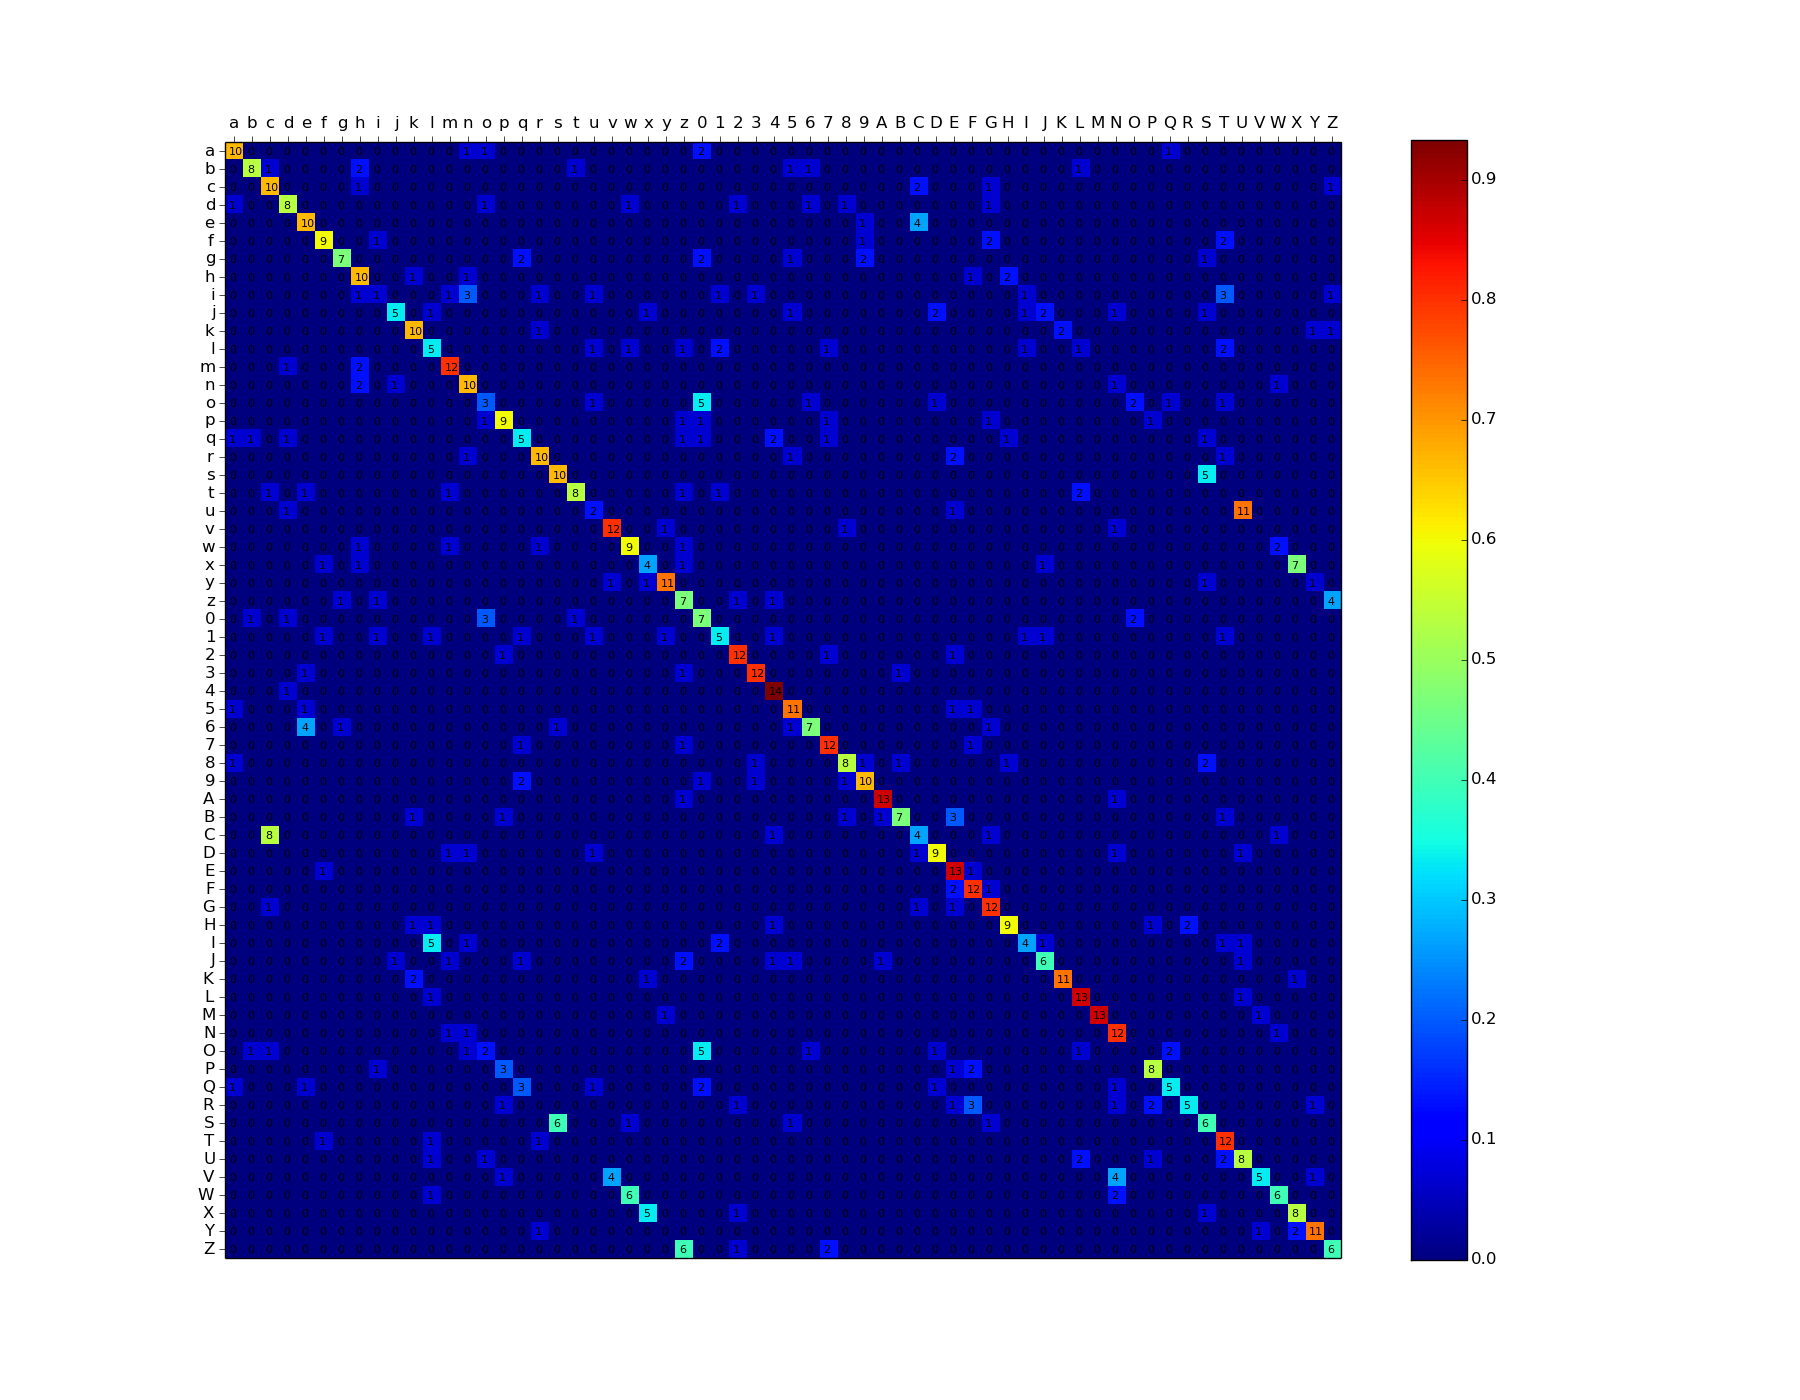
\includegraphics[scale=0.4]{img/resultados/mixtas/best_mean_matrix_Alpha0,01_4080-8.png}}
				\caption[Mixtas Matriz expon]{Matriz de correlación del gráfico \ref{fig: Mixtas-media-mejor} para el mejor resultado. \RC{Demasiado grande las matrices como para mostrarlas y que se vean bien}}
				\label{fig: Mixtas-Matrix-media-mejor}
			\end{figure}
	
			\begin{figure}[!htbp]
				\centerline{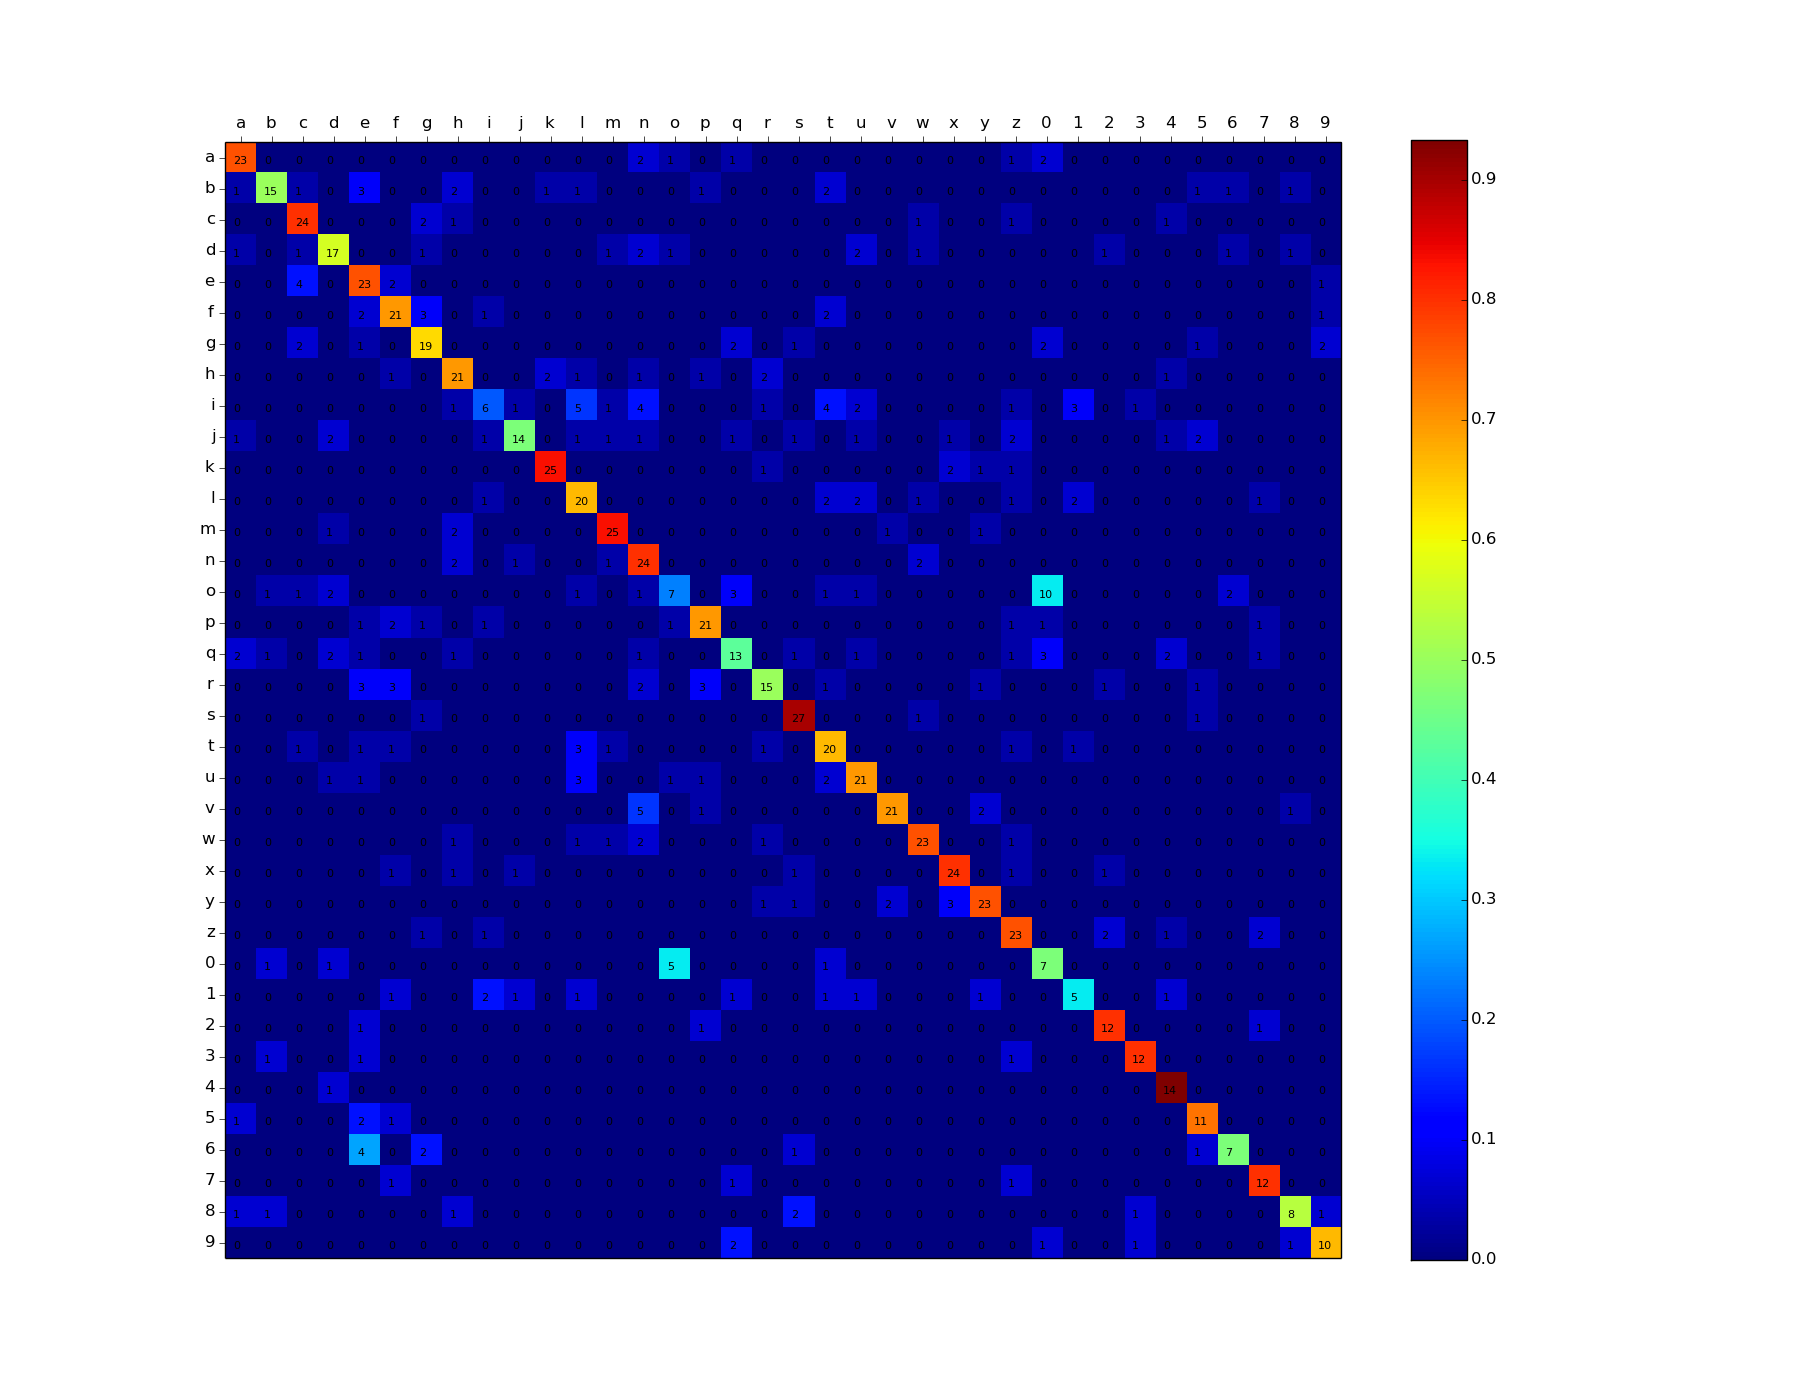
\includegraphics[scale=0.4]{img/resultados/mixtas/best_mean_matrix_Alpha0,01_4080-8_ins.png}}
				\caption[Matriz de correlación ``case insensitive'' para mixtas media]{Matriz de correlación del gráfico \ref{fig: Mixtas-media-mejor} para el mejor resultado no teniendo en cuenta los caracteres en mayúscula.}
				\label{fig: MatrizIns-Mixtas-media-mejor}
			\end{figure}

